
\chapter{Analysis Tools}

\section{Viewing PQR in VMD}

%Load \<yourfile\>\.all\.pqr
Load pqr file
\begin{lstlisting}[style = MyBash]
>> set selall [atomselect top "all"]
\end{lstlisting}

To center the pqr
\begin{lstlisting}[style = MyBash]
>> $selall moveby {-x -y -z}
\end{lstlisting}
where x, y, and z are half the box length

Graphical representations:
To view the charges inside the CG center, from the toolbar, select Graphics \textgreater \,
Representations. In the selected atoms, type
\begin{lstlisting}[style = MyBash]
not name X
\end{lstlisting}

Change the coloring method to Charge, and the Drawing Method to VDW. Then select the 
Create Rep button, and in the selected atoms, type 
\begin{lstlisting}[style = MyBash]
not name X
\end{lstlisting}

 Change the Drawing Method to VDW and the Material to Transparent. 
 The Graphical Representations and final images are in figure below.

\begin{figure}[!htbp]
  \centering
  \begin{minipage}[b]{0.3\textwidth}
    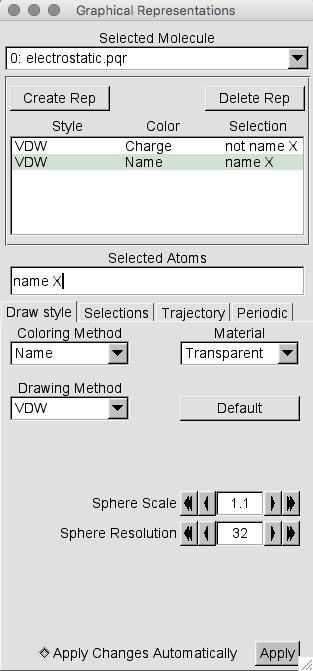
\includegraphics[width=\textwidth]{vmd_graph_rep_pqr}
    \caption{Graphics}
  \end{minipage}
  \hfill
  \begin{minipage}[b]{0.65\textwidth}
    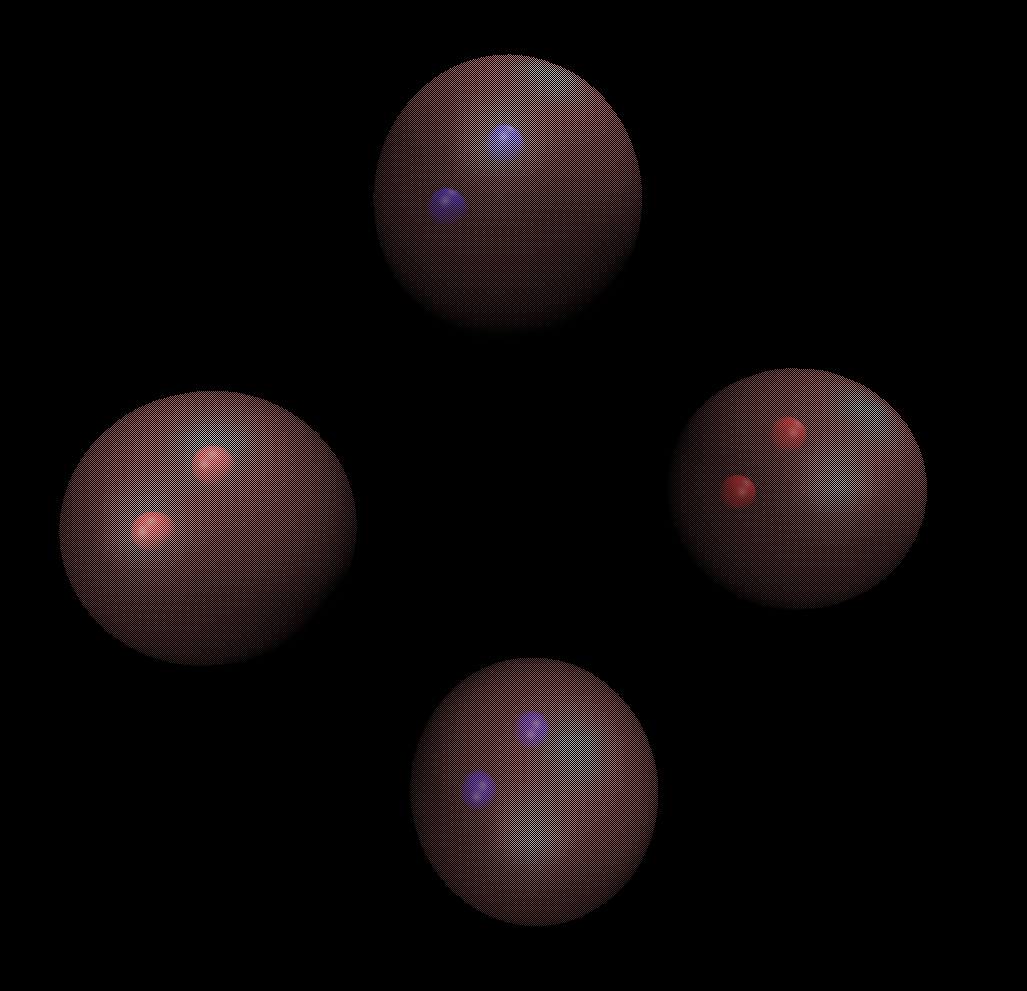
\includegraphics[width=\textwidth]{vmd_4sp}
    \caption{Final view}
  \end{minipage}
\end{figure}

\section{Dynamics tools}
\subsection{Viewing Dynamics in VMD}

First load the PQR file, and then any XYZ files onto the same molecule.

\section{Electrostatics tools}
\subsection{Viewing Electrostatics in VMD}

To load electrostatic results: File \textgreater \, New Molecule. In the window that appears, toggle the \textit{Load files for:} 
to select the currently loaded PQR file. Then select \textit{Browse} to find the location of the dx file. Once found, hit 
the \textit{Load} button and let the dx file load.

\begin{figure}[!htbp]
  \centering
  \begin{minipage}[b]{0.3\textwidth}
    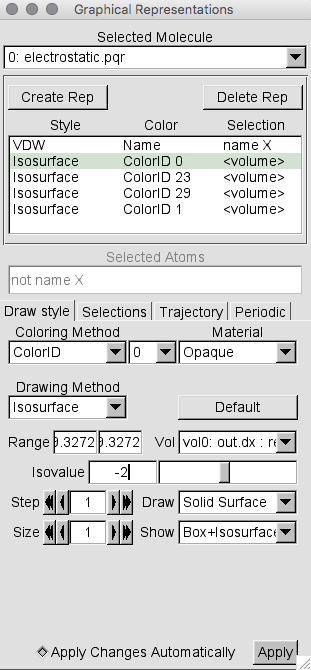
\includegraphics[width=\textwidth]{vmd_graph_rep_dx}
    \caption{DX Graphics}
  \end{minipage}
  \hfill
  \begin{minipage}[b]{0.65\textwidth}
    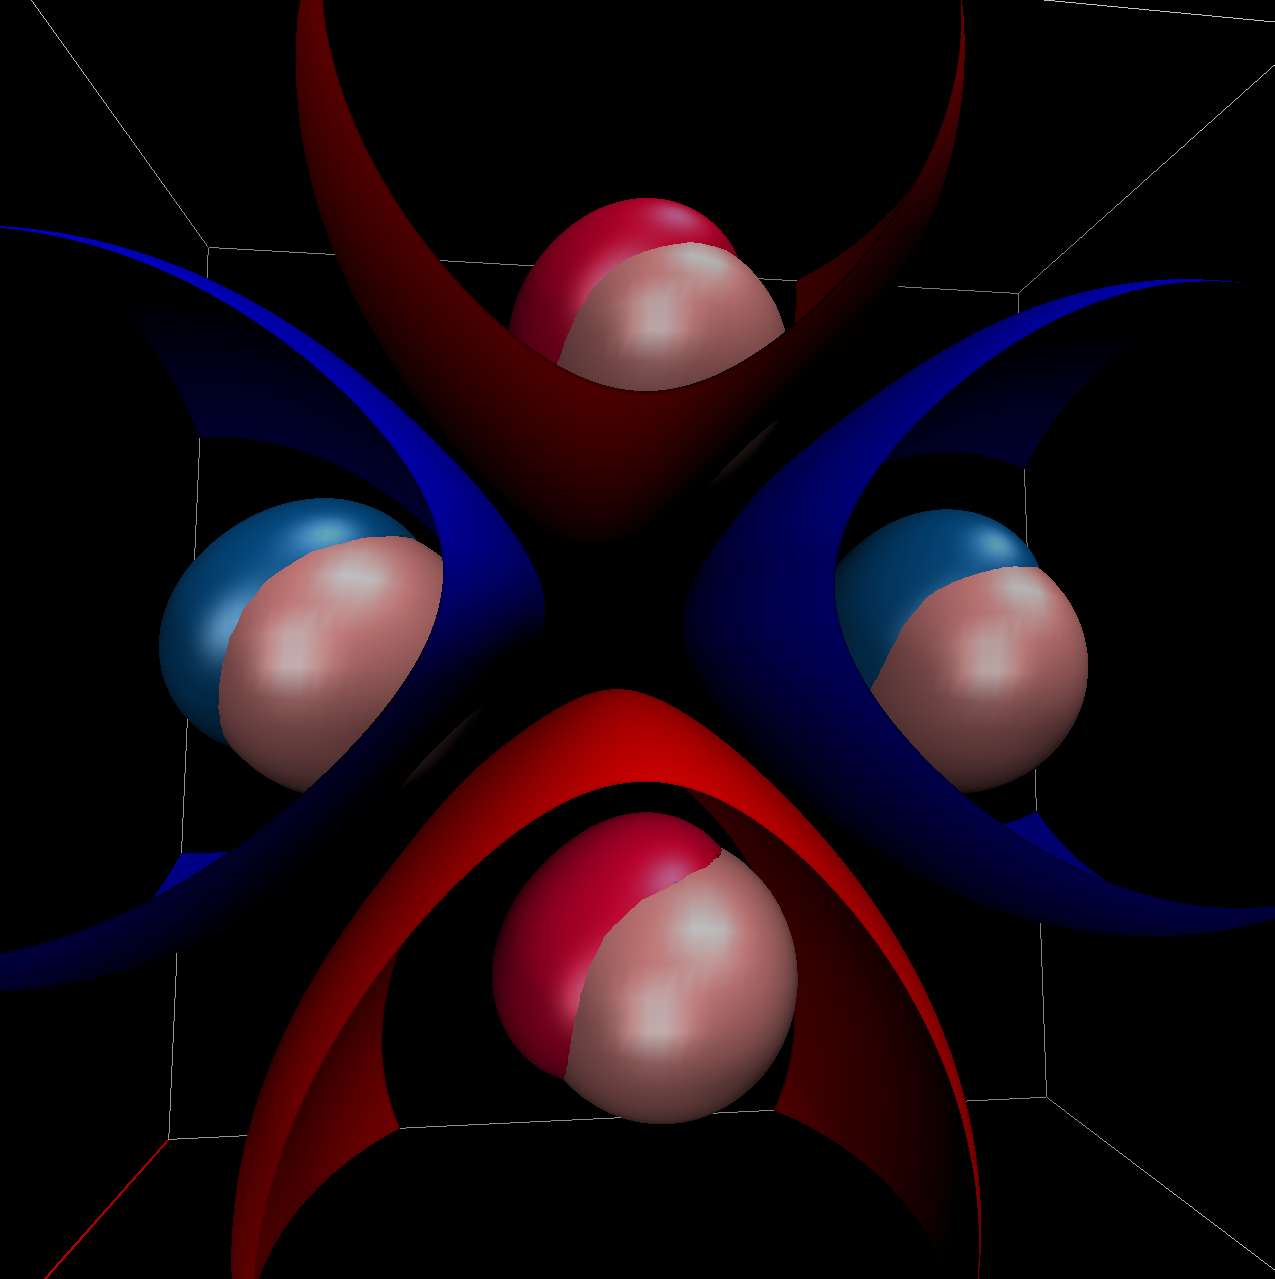
\includegraphics[width=\textwidth]{vmd_4sp_dx}
    \caption{DX representation}
  \end{minipage}
\end{figure}

 \clearpage

%\section{Mean First Passage Time (MFPT)}
%
%collect FPT from complete.dat
%\begin{lstlisting}[style = MyBash]
%	>> cat <yourpath>/complete.dat | awk '{print $7}' >  fpt.txt
%\end{lstlisting}
%run lognorm.py 
%\begin{lstlisting}[style = MyBash]
%	>> python lognorm.py  <yourpath>/fpt.txt
%\end{lstlisting}
%The final line of the output gives average and standard deviation for first passage times
%based on the lognormal probability distribution.
%The other lines output shape parameters describing the skew and kurtosis of the PDF
%It can also plot the histogram of FPT.
%
%
%To Do : get diffusion constant from fpt.txt as well


\subsection{2D ESP plots}
From the electrostatic option in PB-AM, a file is created with the following format: \\

\begin{lstlisting}[style = MyBash]
# Data from PBAM Electrostat run
# My runname is barnase.x.0.dat
units kT
grid 200 200 
axis x 0 
origin -51.2204 -51.2204
delta 0.512204 0.512204
maxmin 1.35396 0
   0.2352107     0.2360552     0.2368904     0.2377159
\end{lstlisting}

\medskip

In our \texttt{tools} directory we have provided a python script for plotting this potential.
Change filename within .py file, and the desired output name.
\begin{lstlisting}[style = MyBash]
>> python potential_plot
\end{lstlisting}

\medskip

creates a JPG file of the cross sectioned potential, like the one given below:

\begin{figure}[!htbp]
  \centering
    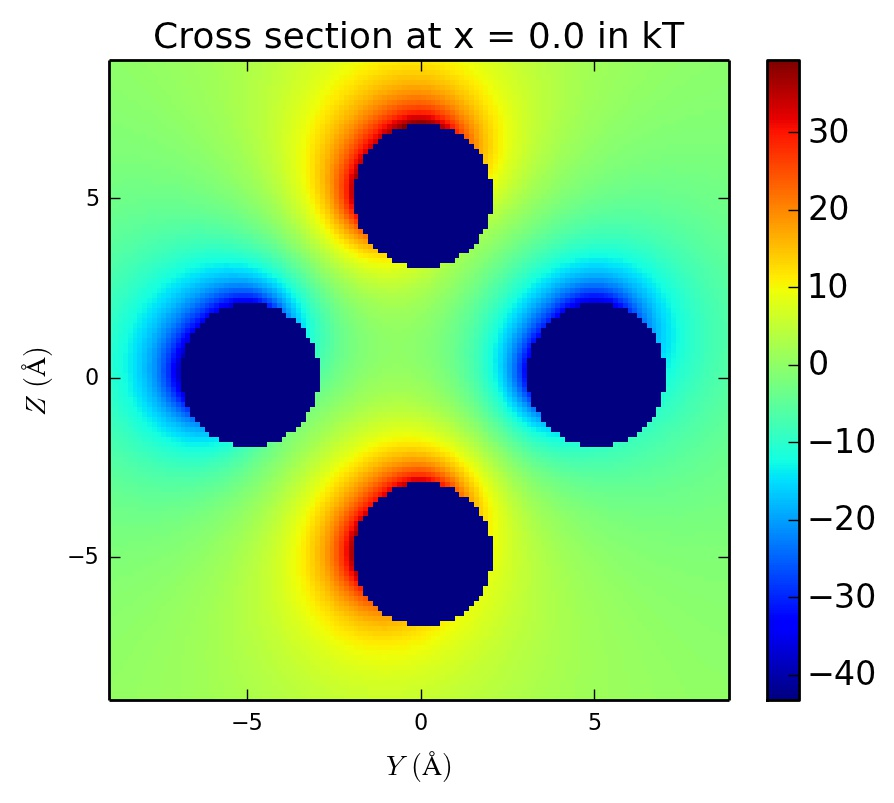
\includegraphics[scale=0.3]{pot_x_0}
    \caption{Potential plot}
\end{figure}

\subsection{3D ESP plots}
From the electrostatic option in PB-AM, a file is created with the following format: \\

\begin{lstlisting}[style = MyBash]
# Data from PBAM Electrostat run
# My runname is electro_map.out and units kT
grid 10 10 10
origin -4 -9 -9
delta 0.8 1.8 1.8
  0.00000   0.00000  -2.90000 -5.899581 
\end{lstlisting}

\medskip

In our \texttt{tools} directory we have provided a python script for plotting this potential.
Change filename within .py file, and the desired output name.
\begin{lstlisting}[style = MyBash]
>> python plot_3d_surf
\end{lstlisting}

\medskip

creates many JPG files of the cross sectioned potential, like the one given below:

\begin{figure}[!htbp]
  \centering
    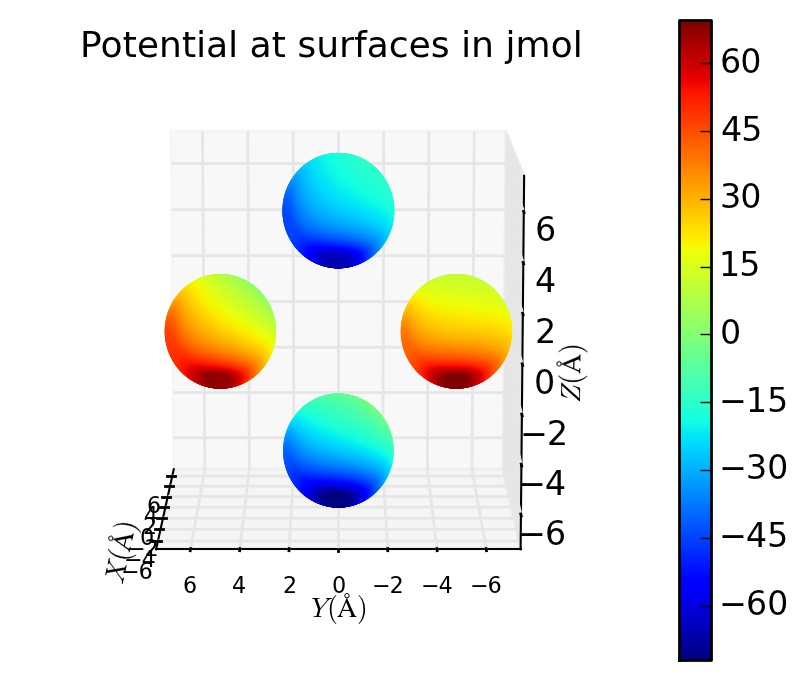
\includegraphics[scale=0.4]{4sp_surf}
    \caption{Molecule surface potential plot}
\end{figure}

	
%\section{Comparison of Displacement Due to Electrostatics versus Diffusion}	
%
%Because Brownian dynamics directly calculated displacements, 
%it is easier to compare relative displacements rather than relative forces.
%
%Separate the displacements due to Electrostatics and Diffusion into their own files.
%In the same directory as bdtest.out :
%\begin{lstlisting}[style = MyBash]
%	>> bash cfDisplacements.sh
%\end{lstlisting}
%Currently set to use only the final completed trajectory in bdtest.out
%This creates two files : dispES.out and dispRand.out
%In the same directory:
%\begin{lstlisting}[style = MyBash]
%	>> python avgDisp.py
%\end{lstlisting}
%This outputs the average displacement in Angstroms due to electrostatics and diffusion, in that order.
%
%
%
%\section{Length Scaling of FPT}
%
%How does the MFPT change with arbitrary choice of length scale?
%
%\begin{lstlisting}[style = MyBash]
%	>> bash lengthScale.sh
%\end{lstlisting}
%
%This script re-analyzes the trajectory for FPT with distances of 10, 20, ... \AA{}.




